\documentclass{beamer}
%
% Choose how your presentation looks.
%
% For more themes, color themes and font themes, see:
% http://deic.uab.es/~iblanes/beamer_gallery/index_by_theme.html
%
\mode<presentation>
{
  \usetheme{Warsaw}      % or try Darmstadt, Madrid, Warsaw, ...
  \usecolortheme{default} % or try albatross, beaver, crane, ...
  \usefonttheme{default}  % or try serif, structurebold, ...
  \setbeamertemplate{navigation symbols}{}
  \setbeamertemplate{caption}[numbered]
}
\usepackage[L7x]{fontenc}
\usepackage{caption}
\usepackage{lmodern} 
%%%%movie%%%
\setbeamertemplate{itemize items}[circle]

%%%%%%%%%%%%%%%%%%%%%5
\usepackage{multimedia}
\usepackage{animate}

\usepackage{envmath}
%\usepackage{amsmath,amssymb}
\usepackage{cancel}
\usepackage{graphicx}
\usepackage{epsfig}
\usepackage{amsmath,amsfonts,amssymb}
\usepackage{natbib}

\usepackage[T1]{fontenc}
\usepackage[english]{babel}
\usepackage{hyphenat}
\hyphenation{mate-mática recu-perar}
\bibliographystyle{unsrtnat}
\usepackage{tabularx} % extra features for tabular environment
\usepackage{amsmath}  % improve math presentation
\usepackage{blindtext}
%\usepackage{enumitem} tirar isto no beamer
\usepackage{xcolor}
\usepackage{graphicx} % takes care of graphic including machinery
\usepackage{graphics} 
\usepackage{float}
%\usepackage[margin=1in,letterpaper]{geometry}% decreases margins
%\usepackage{cite} % takes care of citations

\usepackage{lipsum}
\usepackage{mwe}
 \newcommand{\sign}{\mathop{\mathrm{sign}}}

\graphicspath{{images/}}
\usepackage{cases}

%%%%%%%%%%%%%%%%%%%%%%%%5

\usepackage[english]{babel}
\usepackage[utf8x]{inputenc}

\title[TAFC]{Bipedal Walking using a Spring Mass model}
%\author{Nuno Teixeira nº 75494}
\author[Nuno Teixeira]{Nuno Teixeira nº 75494}
\institute{Instituto Superior Técnico}
\date{\today}
\setbeamersize{text margin left=0.5cm,text margin right=0.5cm}


\addtolength{\headsep}{0.6cm}


\begin{document}

\begin{frame}
  \titlepage
\end{frame}

\section{Introduction}
\begin{frame}{Walking model}
  \begin{center}
  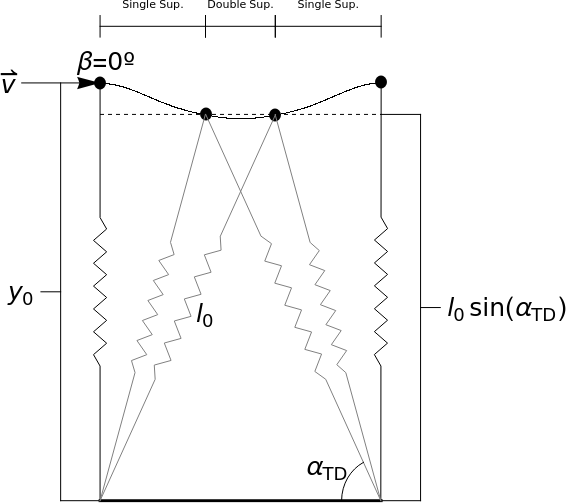
\includegraphics[height=0.5\textheight]{Seyfarth2006_trimmed.png}
  \end{center}
Definitions:
  \begin{itemize}
\item  \underline{stride} - Leg crosses the vertical leg orientation
\item  \underline{step} -The moment when the system passes from single support to double support.
  \end{itemize}
\end{frame}

\begin{frame}{Equations}

  \begin{block}{Single support}
  \begin{equation}
  \ddot{x}=\frac{F_1}{m}\frac{x-x_{t1}}{l_1}
  \label{eq.singlesuppx}
  \end{equation}
\begin{equation}
  \ddot{y}=\frac{F_1}{m}\frac{y-y_{t1}}{l_1}-g
  \label{eq.singlesuppy}
\end{equation}
\end{block}

  \begin{block}{Double support}
\begin{equation}
 \ddot{x}=\frac{F_1}{m}\frac{x-x_{t1}}{l_1}+\frac{F_2}{m}\frac{x-x_{t2}}{l_2}
 \label{eq.doublesuppx}
  \end{equation}
\begin{equation}
  \ddot{y}=\frac{F_1}{m}\frac{y-y_{t1}}{l_1}+\frac{F_2}{m}\frac{y-y_{t2}}{l_2}-g
  \label{eq.doublesuppy}
\end{equation}
\end{block}

\end{frame}

\begin{frame}

with $F_i$ being the force applied on the mass by the respective leg,
\begin{equation}
  F_i=k(l_0-l_i)\geq 0 \,\,\,\,\, i=1,2\,,
\end{equation}
$l_0$ is the natural length of the spring, $l_i$ is the respective length,
\begin{equation}
l_i=\sqrt{(x-x_{ti})^2+(y-y_{ti})^2} \,\,\,\,\, i =1,2 \,.
\end{equation}

Since the system is energetically conservative we can change the initial velocity by inverting
  \begin{equation}
  E=\frac{k (l_0-y_0)^2}{2} + m g y_0 + m \frac{v_0^2}{2}.
\end{equation}

\end{frame}

\section{Method}
\begin{frame}{Parameters}

    \begin{block}{A scan is made with 3 parameters, $Energy$, $y_0$, $\alpha$ in two strides}
    \begin{itemize}
\item $Energy \in  [800,840]$ with 40 subdivisions.

\item  $\alpha \in [\pi/2-\pi/5,\pi/2]$ with 30 subdivisions.

\item  $y_0 \in [l_0\sin(\alpha) ,l_0]$ with 25 subdivisions
    \end{itemize}
\end{block}
  In all simulations the following parameters remained fixed.
  \begin{itemize}
    
\item $\beta=0$
  
\item  $m=80 Kg$
  
\item $l_0=1 m$

\item  $k=14000$

 \end{itemize}

Total number of configurations= $40 \times 30 \times 25 = 30000$

 
\end{frame}

\begin{frame}{Failure conditions}
  With Eqs. (\ref{eq.singlesuppx})-(\ref{eq.doublesuppy}) a fourth order Runge-Kutta was applied to know the position and velocity of the system throught time. Different time steps were applied for different ends.
  
  Not all solutions are admited, solutions in which
  \begin{itemize}
  \item The center of mass starts propagating backward ($v_x<0$)
  \item The center of mass falls ($y<0$)
  \item The center of mass jumps ($y>l0$)  
  \end{itemize}
  were excluded.
  \end{frame}
\begin{frame}{Defining the map}
  Defining $\psi_n=(y_n,\Delta x_n)$ at the stride $n$, and letting $A$ integrate $\psi_n$ to the next step,
  \begin{equation}
    \psi_{n+1}=A \psi_n,
  \end{equation}
  We are interested in obtaining the fixed points of the system with 2 strides.
  We can calculate the fixed points by assigning a map with the parameters from the first step and second step
\end{frame}

\begin{frame}{Fixed points obtention}
  To obtain the fixed points the following steps were done:
  \begin{enumerate}
    \item A configuration parameter point simulation that completed 2 strides was determined  with a Runge-Kutta step of $\Delta t= 0.001$s
 \item A third degree interpolation of the positions and velocities was made.
 \item From this interpolation an interception with the position of the respective toe was done
 \item Register $y_1$, $y_2$, $\Delta x_1$ $\Delta x_2$.
  \end{enumerate}
  
  If  $|\Delta x_2-\Delta x_1|< 0.001$, $|(y_1-y_0)|<0.001$ and $(y_2-y_1)|<0.001$

  then that set of parameters is considered a fixed point of the system 
\end{frame}

\begin{frame}{Stability}
  Obtaining the fixed points, we calculate the jacobian
  \begin{equation}
 J= \begin{bmatrix}
    \frac{\partial \Delta x_{n+1}}{\partial \Delta x_{n}} & \frac{\partial \Delta x_{n+1}}{\partial  y_{n}}\\
     \frac{\partial  y_{n+1}}{\partial \Delta x_{n}} & \frac{\partial y_{n+1}}{\partial  y_{n}}
  \end{bmatrix},
  \label{eigeneq}
  \end{equation}

  with,

  \begin{equation}
    \frac{\partial \Delta x_{n+1}}{\partial \Delta x_{n}}=  \frac{\frac{\partial \Delta x_{n+1}}{\partial t}}{\frac{\partial \Delta x_{n}}{\partial t}}. 
  \end{equation}

  If the eigenvalues of the jacobian in (\ref{eigeneq}), $\lambda_{1,2}$ satisfy $|\lambda_{1,2}|<1$ then the calculated fixed points are stable, otherwise they are unstable.
\end{frame}

\begin{frame}{Survival step configurations}
  Out of the 30000 configurations in the parameter space, only 8195 were able to complete 2 strides. Of this subset of points, 11 fixed points were found, 5 stable and 6 unstable.
  
  From here a survival test is applied to each of the 8195 configurations that completed 2 strides by incrementing steps instead of strides.

  If the simulation fails, the maximum number of steps was assigned to that configuration.
\end{frame}

\section{Results}
\begin{frame}{Fixed points and 10 step configurations}
  Iterating the number of steps where $\Delta t=0.00075$ so that in maximum it was possible to achieve 10 steps, the configurations that achieve 10 steps can be ilustrated in the figure below along with the fixed points.
  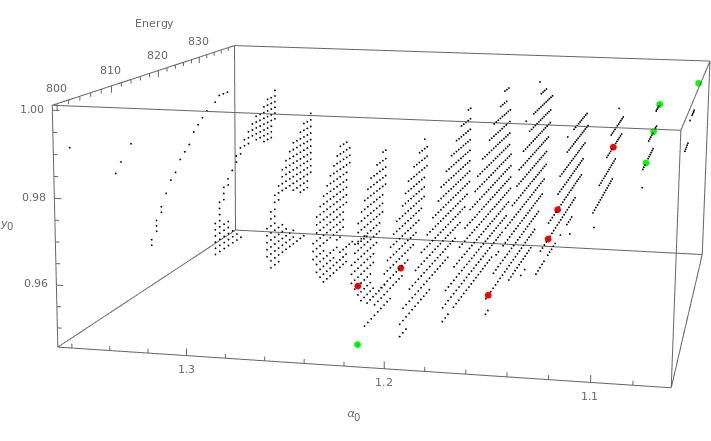
\includegraphics[width=0.8\textwidth]{newfixedpoints.png}


\end{frame}

\begin{frame}{Stable configuration}
  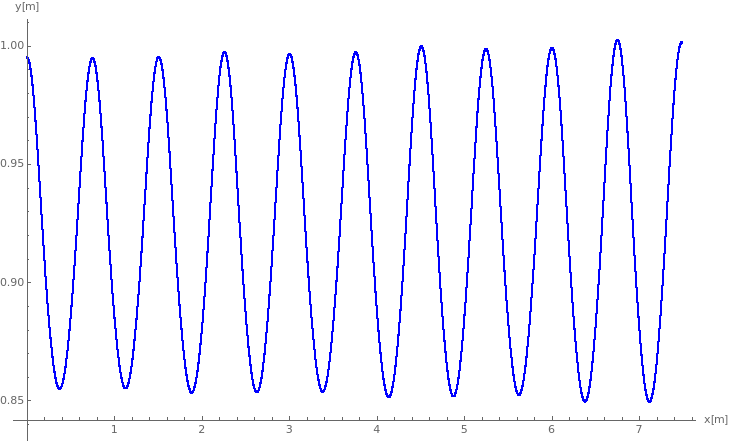
\includegraphics[width=0.8\textwidth]{Stable10steps.png}
  
  E=839J, $\alpha_0$= 1.068,$y_0$=0.995, Runge-Kutta timestep $\Delta t=0.0005$s
\end{frame}

\begin{frame}{Unstable configuration}
  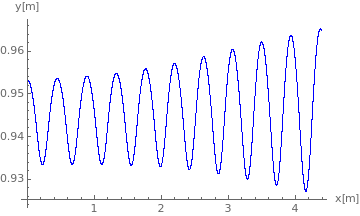
\includegraphics[width=0.8\textwidth]{unstableconfiguration.png}
  
   E=812J, $\alpha_0$= 1.236,$y_0$=0.953, Runge-Kutta timestep $\Delta t=0.0005$s
  
\end{frame}
\section{Conclusions}
\begin{frame}{Conclusions}
  \begin{itemize}    
 \item  Picking the right Runge-Kutta timestep was important, otherwise the system would gain energy indefinitely and would appear to be unstable.
 \item  In the range from 800 to 840 J, the bigger the energy the more configurations were accessible
 \item  The fixed points from $\alpha \in [1,1,22]$ appear to be situated on a plane
   \item It is necessary to broad the range of the parameters so more information can be taken out of the characteristics of stable walking
\end{itemize}
  \end{frame}
\end{document}
